\documentclass[a4paper, english]{article}
\usepackage{graphics,eurosym,latexsym}
\usepackage{listings}
\usepackage{pst-all}
\usepackage{algorithmic,algorithm}
\lstset{columns=fixed,basicstyle=\ttfamily,numbers=left,numberstyle=\tiny,stepnumber=5,breaklines=true}
\usepackage{times}
\usepackage{babel}
\usepackage[useregional]{datetime2}
\usepackage[round]{natbib}
\bibliographystyle{plainnat}
\oddsidemargin=0cm
\evensidemargin=0cm
\newcommand{\be}{\begin{enumerate}}
\newcommand{\ee}{\end{enumerate}}
\newcommand{\bi}{\begin{itemize}}
\newcommand{\ei}{\end{itemize}}
\newcommand{\I}{\item}
\newcommand{\ty}{\texttt}
\textwidth=16cm
\textheight=23cm
\begin{document}
\title{\ty{Epos} v1.1
: Estimating Population Sizes and Allele Ages from
  Site Frequency Spectra}
\author{Bernhard Haubold\\\small Max-Planck-Institute for Evolutionary
  Biology, Pl\"on, Germany}
\date{\input{date}}
\maketitle
\section{Introduction} 
The software package \ty{epos} contains two programs, \ty{epos}
itself and \ty{epos2ages}. \ty{Epos} estimates historical population
sizes, and \ty{epos2ages} transforms them into allele ages. \ty{Epos} takes site frequency spectra as input. A site frequency
spectrum is computed from a haplotype sample. Table~\ref{tab:hap}
shows a sample of $n=4$ haplotypes, $h_1, h_2,...,h_4$, with $S=8$
segregating (polymorphic) sites, $s_1, s_2,...,s_8$. Each segregating
site consists of a column of four zeros and ones, where zero indicate
the ancestral state and one a mutation. We can count the number of
sites where one, two, or three haplotypes are mutated. This is called
the site frequency spectrum (SFS) of the sample, and
Table~\ref{tab:sfs}A shows the spectrum for our example data. There
are seven mutations affecting a single haplotype (singletons), zero
mutations affecting two haplotypes (doubletons), and one mutation
affecting three haplotypes (tripleton).
\begin{table}
  \caption{Four example haplotypes}\label{tab:hap}
  \begin{center}
    \begin{tabular}{lcccccccc}\hline
haplotype   &   $s_1$ & $s_2$ & $s_3$ & $s_4$ & $s_5$ & $s_6$ & $s_7$ & $s_8$\\\hline
$h_1$ &      \ty{1} & \ty{0} & \ty{0} & \ty{0} & \ty{0} & \ty{0} & \ty{0} & \ty{0}\\
$h_2$ &      \ty{0} & \ty{1} & \ty{0} & \ty{0} & \ty{1} & \ty{0} & \ty{0} & \ty{1}\\
$h_3$ &      \ty{0} & \ty{1} & \ty{0} & \ty{1} & \ty{0} & \ty{1} & \ty{0} & \ty{0}\\
$h_4$ &      \ty{0} & \ty{1} & \ty{1} & \ty{0} & \ty{0} & \ty{0} & \ty{1} &
      \ty{0}\\\hline
      \end{tabular}
  \end{center}
\end{table}
In many empirical data sets it is not possible to distinguish between
segregating sites with $r$ mutations and those with $n-r$
mutations. In this case the spectrum is called \textit{folded} and
consists of the
number of sites affecting $r$ haplotypes plus the number of sites
affecting $n-r$ haplotypes. Table~\ref{tab:hap}B shows the folded
version of the spectrum in Table~\ref{tab:hap}A: The singleton
category now consists of the sum of unfolded singletons and
tripletons, while the number of doubletons
remains unchanged.
In addition to population sizes, \ty{epos} can also compute the
average ages of mutations affecting $1, 2,...,n-1$ haplotypes.

\begin{table}
  \caption{Folded (\textbf{A}) and unfolded (\textbf{B}) site
    frequency spectrum corresponding to the haplotype sample shown in Table~\ref{tab:hap}}\label{tab:sfs}
  \begin{center}
  \begin{tabular}{cc}
    \textbf{A} & \textbf{B}\\
    \begin{tabular}{cc}
      \hline
      $r$ & $f(r)$\\\hline
      1 & 7\\
      2 & 0\\
      3 & 1\\\hline
    \end{tabular}
    &
    \begin{tabular}{cc}
      \hline
      $r$ & $f(r)$\\\hline
      1 & 8\\
      2 & 0\\
      \hline
    \end{tabular}
  \end{tabular}
  \end{center}
\end{table}

\section{Theory \& Algorithm}\label{sec:alg}
\ty{Epos} implements theory by \cite{lyn18:inf}. Here I give a non-technical introduction. Consider the
coalescent for $n$ haplotypes; Figure~\ref{fig:coa} shows an example
for $n=4$ haplotypes. Any such coalescent can be divided into levels
$2, 3,...,n$, where a level, $\ell$, is the coalescence event,
where the number of lineages changes from $\ell+1$ to $\ell$. The time
intervals $T_i, 2\le i\le n-1$ denote the segment with $i$
lineages. For each $T_i$ \ty{epos} can calculate a corresponding
population size, $N_i$. Unfortunately, for larger sample sizes the
computation of all $N_i$ invariable returns negative population
sizes. So instead of allowing the population size to change at every
coalescence event, we pick a subset of events encapsulating the most
important size changes.

\begin{figure}
  \begin{center}
    \begin{pspicture}(-1.5,0)(2.5,2.75)
  \psset{xunit=0.25,yunit=0.25}
  \rput( 0.00, 0.00){\Rnode{1}{$h_1$}}
  \rput( 3.33, 0.00){\Rnode{2}{$h_2$}}
  \rput( 6.67, 0.00){\Rnode{3}{$h_3$}}
  \rput(10.00, 0.00){\Rnode{4}{$h_4$}}
  \rput( 1.67, 3.09){\Rnode{5}{}}
  \rput( 5.00, 2.43){\Rnode{6}{}}
  \rput( 8.33, 8.57){\Rnode{7}{}}
  
  \ncline[nodesepA=2pt]{1}{5}
  \ncline[nodesepA=2pt]{2}{6}
  \ncline[nodesepA=2pt]{3}{6}
  \ncline{6}{5}
  \ncline{5}{7}
  \ncline[nodesepA=2pt]{4}{7}

  \rput(-2, 11){$T_i$, $N_i$}
  \rput(12, 11){Level}

  \rput(-2, 0.00){\Rnode{ 8}{}}
  \rput(-2, 2.43){\Rnode{ 9}{}}
  \rput(-2, 3.09){\Rnode{10}{}}
  \rput(-2, 8.57){\Rnode{11}{}}

  \rput(12, 0.00){\Rnode{12}{ 5}}
  \rput(13, 2.43){\Rnode{13}{ 4}}
  \rput(12, 3.09){\Rnode{14}{ 3}}
  \rput(12, 8.57){\Rnode{15}{ 2}}

  \ncline[linestyle=dotted]{8}{12}
  \ncline[linestyle=dotted]{9}{13}
  \ncline[linestyle=dotted]{10}{14}
  \ncline[linestyle=dotted]{11}{15}

  \ncline{<->}{8}{9}\naput{$T_4, N_4$}
  \ncline{<->}{9}{10}\naput{$T_3, N_3$}
  \ncline{<->}{10}{11}\naput{$T_2, N_2$}
\end{pspicture}

  \end{center}
  \caption{A coalescent for $n=4$ haplotypes to illustrate the time
    intervals, $T_i$, the corresponding population sizes, $N_i$, and
    the \emph{levels} in the tree.}\label{fig:coa}
\end{figure}

Each combination of levels must contain level 2, the root. If no
further level is added, $N_2$ is computed, the population size for the
whole coalescent. Similarly, breakpoints at levels 2 and 4 would mean
that there is one population sizes for $T_2$ and $T_3$, and another
population size for $T_4$.

So, given a combination of levels, the population sizes are computed
with the proviso that negative values are set to the smallest possible
population size, $N=1$. For each combination of levels and population
sizes, the log-likelihood of observing the input site frequency
spectrum is calculated. We now need an efficient and effective method
for maximizing this likelihood.

The starting point is always a single level, $m=1$, the root at level
2. Then all level pairs $(2,3), (2,4),...,(2,n)$ are examined and the
most likely combination picked. If this improves the likelihood by at
least 2 units, the number of levels is increased to $m=3$ and the
search repeats. Algorithm~\ref{alg:epo} summarizes this strategy. The
function \ty{nextConfig} in line 7 hides the details of how the next
configuration is picked. Here I have implemented a \emph{greedy} and
an \emph{exhaustive} strategy. Under the greedy strategy, the best
configuration of breakpoints found in round $m$ is retained in round
$m+1$ and a single new breakpoint is added. Under the exhaustive
strategy, all ${n-1\choose m-2}$ possible combinations of breakpoints
are investigated in each round. Unfortunately, for large samples, this
number quickly leads to unfeasible run times. The greedy and
exhaustive search strategies are contrasted in the Tutorial in
Section~\ref{sec:tut}, where I also apply \ty{epos} to real site
frequency spectra.

\begin{algorithm}
  \caption{Searching for break points in the coalescent}\label{alg:epo}
  \begin{algorithmic}[1]
  \REQUIRE{$n$} \COMMENT{Sample size}
  \REQUIRE{$\mathrm{f}$} \COMMENT{Array of $n-1$ or $n/2$ site frequencies, the
  unfolded or folded site frequency spectrum, SFS}
  \ENSURE{$m$} \COMMENT{Number of estimated population sizes}
  \ENSURE{$\mathrm{k}$} \COMMENT{Array of $m$ population size change points}
  \ENSURE{$\mathrm{N}$} \COMMENT{Array of $m$ population sizes at
    change points $\mathrm{k}[i], i=1,2,...,m$}
  \STATE{$m\leftarrow 1$} \COMMENT{Initialize to one population size...}
  \STATE{$\mathrm{k}[m]\leftarrow 2$} \COMMENT{...which starts at the root}
  \STATE{$\mathrm{N}\leftarrow \ty{popSizes}(m, \mathrm{k}, \mathrm{f})$}
  \COMMENT{Size of constant population}
  \STATE{$l\leftarrow\ty{likelihood}(\mathrm{N}, m, \mathrm{k},
    \mathrm{f})$} \COMMENT{Likelihood of population size given the SFS}
  \STATE{$l_{\rm a}\leftarrow l$} \COMMENT{The initial likelihood is
    also the maximum}
  \FOR{$m\leftarrow 2$ to $n$} 
     \WHILE{$(\mathrm{k}'\leftarrow\ty{nextConfig}(m, n))\ne\mathrm{null}$} 
        \STATE{$\mathrm{N}'\leftarrow\ty{popSizes}(m, \mathrm{k}',
          \mathrm{f})$}
        \STATE{$l'\leftarrow\ty{likelihood}(\mathrm{N}', m, \mathrm{k}',
          \mathrm{f})$}
        \IF{$l'>l_{\rm a}$}
           \STATE{$\mathrm{k}_{\rm a}\leftarrow\mathrm{k}'$}
           \STATE{$\mathrm{N}_{\rm a}\leftarrow\mathrm{N}'$}
           \STATE{$l_{\rm a}\leftarrow l'$}
        \ENDIF
     \ENDWHILE
     \IF{$l_{\rm a} < l+2$}
        \STATE{$\ty{report}(\mathrm{N}, \mathrm{k}, m-1)$}
        \STATE{$\ty{break}$}
     \ENDIF
     \STATE{$\mathrm{k}\leftarrow \mathrm{k}_{\rm a}$}
     \STATE{$\mathrm{N}\leftarrow \mathrm{N}_{\rm a}$}
     \STATE{$l\leftarrow l_{\rm a}$}
  \ENDFOR
\end{algorithmic}

\end{algorithm}

\section{Getting Started}
\ty{Epos} was written in C on a computer running Linux. It depends on
two libraries, the Gnu Scientific Library
(\ty{lgsl}), and the Basic Linear Algebra Subprograms (\ty{lblas}). 
Please contact \ty{haubold@evolbio.mpg.de} if there are any problems with the program.
\bi
\I Obtain the package
\begin{verbatim}
git clone https://www.github.com/evolbioinf/epos
\end{verbatim}
\I Change into the directory just downloaded
\begin{verbatim}
cd epos
\end{verbatim}
and make the programs \ty{epos} and \ty{epos2ages}
\begin{verbatim}
make
\end{verbatim}
\I Test both programs
\begin{verbatim}
make test
\end{verbatim}
\I The executables \ty{epos} and \ty{epos2ages} are located in the
directory \ty{build}. Place them in your \ty{PATH}.
\I  Make the documentation
\begin{verbatim}
make doc
\end{verbatim}
This calls \LaTeX{}, so document construction depends on a reasonably
complete \ty{latex} installation. The typeset documentation is located
in
\begin{verbatim}
doc/epos.pdf
\end{verbatim}
\ei

\section{Tutorial}\label{sec:tut}
I first explain how to test \ty{epos} using simulated data, and then
analyze real data.
\subsection{Simulated Data}
\ty{Epos} was developed for estimating variable population
sizes. Nevertheless, we begin by simulating simple constant-size
scenarios before generating samples under models with varying population
sizes.
\subsubsection{Constant Population Size}
\begin{itemize}
\item Simulate one sample with
  $n=30$ haplotypes using the coalescent simulator \ty{ms} \citep{hud02:gen}:
\begin{verbatim}
ms 30 1 -t 10 
\end{verbatim}
This can automatically be converted to site frequency spectra using
my program \ty{ms2sfs}\footnote{\ty{https://www.github.com/evolbioinf/sfs}}:
\begin{verbatim}
ms 30 1 -t 10 | ms2sfs
\end{verbatim}
Finally, \ty{epos} then reads the spectrum and estimates population
sizes from it:
\begin{verbatim}
ms 30 1 -t 10 | ms2sfs | tee tmp.sfs | epos -U -l 1000
#InputFile:	stdin
#Polymorphic sites surveyed:	80
#Monomorphic sites surveyed:	920
#m = 1; maximum Log(Likelihood): 5375.211460	{2}
#m = 2; maximum Log(Likelihood): 5381.027523	{2, 5}
#m = 3; maximum Log(Likelihood): 5382.600833	{2, 3, 5}
#Final        Log(Likelihood): 5381.027523
#Level  T[Level]  N[Level]
5       4.20e+05  4.84e+05
2       5.24e+06  1.61e+06
\end{verbatim}
where \ty{-U} indicates an unfolded site frequency spectrum, and
\ty{-l} is the sequence length, $l=1000$. The command \ty{tee} saves
the spectrum in \ty{tmp.sfs} so we can use it again later on.
\ty{Epos} prints intermediate configurations of $m$ breakpoints: As
already described in Section~\ref{sec:alg}, it starts with a single
breakpoint, $m=1$, the root at at level 2. The root level must always
be present and the population size starting there extends to the next
breakpoint printed, or, if there is none as in this case, the
leaves. The log-likelihood of the input site frequency spectrum given
the best-fitting constant population size, which \ty{epos} does not
show, is 5375.2. In the next round, $m=2$, one new breakpoint is added
at level 5. The log-likelihood increases to 5381.0, which is more than
2 units greater than the previous log-likelihood, so the search is
continued in round $m=3$. The breakpoint at level 5 from the previous
round is retained and the next best breakpoint, level 3, is added. The
log-likelihood grows to 5682.6, an increment of less than 2, so the
addition of level 3 is rejected and the result from the previous round
printed. This search strategy is \emph{greedy}, because it cannot
revise the level configurations found in previous rounds.

As an alternative to the greedy strategy, I have also implemented an
exhaustive search, where all possible combinations are tested in each
round. This mode is switched on using $\ty{-E}\ n$, meaning up to $n$
rounds of exhaustive search are conducted before the program reverts
to the greedy strategy, or quits. Apply the exhaustive strategy to the
data set just analyzed:
\begin{verbatim}
epos -U -l 1000 -E 10 tmp.sfs
#InputFile:	tmp.sfs
#Polymorphic sites surveyed:	80
#Monomorphic sites surveyed:	920
#m = 1; maximum Log(Likelihood): 5375.211460	{2}
#m = 2; maximum Log(Likelihood): 5381.027523	{2, 5}
#m = 3; maximum Log(Likelihood): 5383.636893	{2, 3, 6}
#m = 4; maximum Log(Likelihood): 5385.036300	{2, 3, 6, 27}
#Final        Log(Likelihood): 5383.636893
#Level  T[Level]  N[Level]
6       1.90e+05  2.85e+05
3       3.40e+06  2.68e+06
2       4.35e+06  4.74e+05
\end{verbatim}
Up to $m=2$ the runs are identical. But in $m=3$ the breakpoint at
level 5 is not retained, which opens the way to finding another
significant improvement before giving up in round $m=4$. So the
exhaustive search can lead to better results than the greedy
search. Unfortunately, the exhaustive search requires ${n-1\choose
  m-2}$ steps for each value of $m$ investigated. If $n$ is large, say
200, and $m=10$, the number of steps is ${199\choose 8}\approx
5.3\times10^{13}$, which is an unfeasible number of estimations and
likelihood computations. So in many situations the exhaustive search
is not practical.

\ty{Epos} interprets the population mutation parameter,
$\theta=4N_{\rm e}\mu$, as per-site, which means that under constant
population size the expected effective size is
\[
E[N_{\rm e}]=\frac{\theta}{4\mu l}.
\]
Since \ty{epos} uses by default $\mu=5\times 10^{-9}$, the expected
population size for our simulation data is therefore 500,000. We can
test this by simulating 1000 samples, calculating a site frequency
spectrum for each, and averaging over the estimated population sizes:
\begin{verbatim}
ms 30 1000 -t 10 |              # generate 1000 samples of 30 haplotypes
ms2sfs           |              # compute one spectrum per sample
epos -U -l 1000  |              # estimate population sizes for each spectrum
grep -v '^#'     |              # remove hashed lines
awk '{s+=$3;c++}END{print s/c}' # compute average population size
1.36147e+06
\end{verbatim}
This is almost three times larger than the expected 500,000 and
illustrates that the average is not a good statistic for monitoring
the ``majority'' behavior of \ty{epos} estimates. What about the
median? We repeat the simulation, but this time save the population sizes to
the file \ty{tmp.txt}:
\begin{verbatim}
ms 30 1000 -t 10 |              # generate 1000 samples of 30 haplotypes
ms2sfs           |              # compute one spectrum per sample
epos -U -l 1000  |              # estimate population sizes for each spectrum
grep -v '^#'     |              # remove hashed lines
cut -f 3  > tmp.txt             # extract the third column and save it
\end{verbatim}
Now we count the results:
\begin{verbatim}
wc -l tmp.txt
1568 tmp.txt
\end{verbatim}
and look up the median
\begin{verbatim}
sort -g tmp.txt | head -n 784 | tail -n 1
4.67e+05
\end{verbatim}
which is reasonably close to the expected value of $5\times 10^5$.
Let's see if folding the
spectrum changes this result:
\begin{verbatim}
ms 30 1000 -t 10 | 
ms2sfs -f        |  # fold the spectra 
epos -l 1000     |  
grep -v '^#'     |
cut -f 3         |
sort -g > tmp.txt
\end{verbatim}
Now count the results
\begin{verbatim}
wc -l tmp.txt
1667
\end{verbatim}
and find the median
\begin{verbatim}
head -n 834 tmp.txt | tail -n 1
5.27e+05
\end{verbatim}
which is again similar to the expected 500,000. 
\end{itemize}
\subsubsection{Variable Population Size}
\begin{itemize}
  \item For estimating variable population sizes we need to
    plot size as a function of time. This is implemented in the
    program \ty{epos2plot}\footnote{\ty{https://www.github.com/evolbioinf/epos2plot}}. Begin again by simulating samples under constant population
    size, but this time add plotting
\begin{verbatim}
ms 30 1000 -t 10 | 
ms2sfs           | 
epos -U -l 1000  | 
epos2plot > epos1.dat # generate data ready for plotting
\end{verbatim}
Draw the graph by applying the program
\ty{gnuplot}\footnote{\ty{http://www.gnuplot.info/}} to the file
\ty{fig1.gp}, which is part of the \ty{epos} package:
\begin{verbatim}
gnuplot -p fig1.gp
\end{verbatim}
to get Figure~\ref{fig:con}. The fit between the estimated median size
and the true size is excellent for most of the plot, though it drifts
upward in the very distant past. It is important to realize that the number of samples
from which the estimates are derived declines into the past. Near the
present we have
\begin{verbatim}
head -n 5 epos1.dat 
#Time  LowerQ  Median  UpperQ    SampleSize
0      25300   484000  1.81e+07  1000
128    25300   484000  1.81e+07	 1000
324    26700   489000  1.81e+07	 1000
345    29800   492000  1.81e+07	 1000
\end{verbatim}        
while the furthest point in the past is usually computed from a single
sample:
\begin{verbatim}
tail -n 5 epos1.dat 
6.58e+06  2.34e+06  2.36e+06  2.71e+06  5
6.6e+06   2.34e+06  2.4e+06   2.71e+06  4
7.06e+06  2.34e+06  2.4e+06   2.71e+06  3
7.21e+06  2.4e+06   2.71e+06  2.71e+06  2
7.3e+06   2.71e+06  2.71e+06  2.71e+06  1
\end{verbatim}
Also, the variation in Figure~\ref{fig:con} is
large, especially close to the present.
\begin{figure}
  \begin{center}
    \scalebox{0.6}{% GNUPLOT: LaTeX picture with Postscript
\begingroup
  \makeatletter
  \providecommand\color[2][]{%
    \GenericError{(gnuplot) \space\space\space\@spaces}{%
      Package color not loaded in conjunction with
      terminal option `colourtext'%
    }{See the gnuplot documentation for explanation.%
    }{Either use 'blacktext' in gnuplot or load the package
      color.sty in LaTeX.}%
    \renewcommand\color[2][]{}%
  }%
  \providecommand\includegraphics[2][]{%
    \GenericError{(gnuplot) \space\space\space\@spaces}{%
      Package graphicx or graphics not loaded%
    }{See the gnuplot documentation for explanation.%
    }{The gnuplot epslatex terminal needs graphicx.sty or graphics.sty.}%
    \renewcommand\includegraphics[2][]{}%
  }%
  \providecommand\rotatebox[2]{#2}%
  \@ifundefined{ifGPcolor}{%
    \newif\ifGPcolor
    \GPcolortrue
  }{}%
  \@ifundefined{ifGPblacktext}{%
    \newif\ifGPblacktext
    \GPblacktexttrue
  }{}%
  % define a \g@addto@macro without @ in the name:
  \let\gplgaddtomacro\g@addto@macro
  % define empty templates for all commands taking text:
  \gdef\gplbacktext{}%
  \gdef\gplfronttext{}%
  \makeatother
  \ifGPblacktext
    % no textcolor at all
    \def\colorrgb#1{}%
    \def\colorgray#1{}%
  \else
    % gray or color?
    \ifGPcolor
      \def\colorrgb#1{\color[rgb]{#1}}%
      \def\colorgray#1{\color[gray]{#1}}%
      \expandafter\def\csname LTw\endcsname{\color{white}}%
      \expandafter\def\csname LTb\endcsname{\color{black}}%
      \expandafter\def\csname LTa\endcsname{\color{black}}%
      \expandafter\def\csname LT0\endcsname{\color[rgb]{1,0,0}}%
      \expandafter\def\csname LT1\endcsname{\color[rgb]{0,1,0}}%
      \expandafter\def\csname LT2\endcsname{\color[rgb]{0,0,1}}%
      \expandafter\def\csname LT3\endcsname{\color[rgb]{1,0,1}}%
      \expandafter\def\csname LT4\endcsname{\color[rgb]{0,1,1}}%
      \expandafter\def\csname LT5\endcsname{\color[rgb]{1,1,0}}%
      \expandafter\def\csname LT6\endcsname{\color[rgb]{0,0,0}}%
      \expandafter\def\csname LT7\endcsname{\color[rgb]{1,0.3,0}}%
      \expandafter\def\csname LT8\endcsname{\color[rgb]{0.5,0.5,0.5}}%
    \else
      % gray
      \def\colorrgb#1{\color{black}}%
      \def\colorgray#1{\color[gray]{#1}}%
      \expandafter\def\csname LTw\endcsname{\color{white}}%
      \expandafter\def\csname LTb\endcsname{\color{black}}%
      \expandafter\def\csname LTa\endcsname{\color{black}}%
      \expandafter\def\csname LT0\endcsname{\color{black}}%
      \expandafter\def\csname LT1\endcsname{\color{black}}%
      \expandafter\def\csname LT2\endcsname{\color{black}}%
      \expandafter\def\csname LT3\endcsname{\color{black}}%
      \expandafter\def\csname LT4\endcsname{\color{black}}%
      \expandafter\def\csname LT5\endcsname{\color{black}}%
      \expandafter\def\csname LT6\endcsname{\color{black}}%
      \expandafter\def\csname LT7\endcsname{\color{black}}%
      \expandafter\def\csname LT8\endcsname{\color{black}}%
    \fi
  \fi
    \setlength{\unitlength}{0.0500bp}%
    \ifx\gptboxheight\undefined%
      \newlength{\gptboxheight}%
      \newlength{\gptboxwidth}%
      \newsavebox{\gptboxtext}%
    \fi%
    \setlength{\fboxrule}{0.5pt}%
    \setlength{\fboxsep}{1pt}%
\begin{picture}(7200.00,6720.00)%
    \gplgaddtomacro\gplbacktext{%
      \csname LTb\endcsname%%
      \put(1078,704){\makebox(0,0)[r]{\strut{}\large $10^{5}$}}%
      \put(1078,3601){\makebox(0,0)[r]{\strut{}\large $10^{6}$}}%
      \put(1078,6499){\makebox(0,0)[r]{\strut{}\large $10^{7}$}}%
      \put(1210,484){\makebox(0,0){\strut{}\large $10^{3}$}}%
      \put(2624,484){\makebox(0,0){\strut{}\large $10^{4}$}}%
      \put(4038,484){\makebox(0,0){\strut{}\large $10^{5}$}}%
      \put(5452,484){\makebox(0,0){\strut{}\large $10^{6}$}}%
    }%
    \gplgaddtomacro\gplfronttext{%
      \csname LTb\endcsname%%
      \put(198,3601){\rotatebox{-270}{\makebox(0,0){\strut{}\large $N_{\rm e}$}}}%
      \put(4006,154){\makebox(0,0){\strut{}\large Time (Generations)}}%
      \csname LTb\endcsname%%
      \put(5816,6326){\makebox(0,0)[r]{\strut{}\large 5\% quantile}}%
      \csname LTb\endcsname%%
      \put(5816,6106){\makebox(0,0)[r]{\strut{}\large median}}%
      \csname LTb\endcsname%%
      \put(5816,5886){\makebox(0,0)[r]{\strut{}\large expected}}%
      \csname LTb\endcsname%%
      \put(5816,5666){\makebox(0,0)[r]{\strut{}\large 95\% quantile}}%
    }%
    \gplbacktext
    \put(0,0){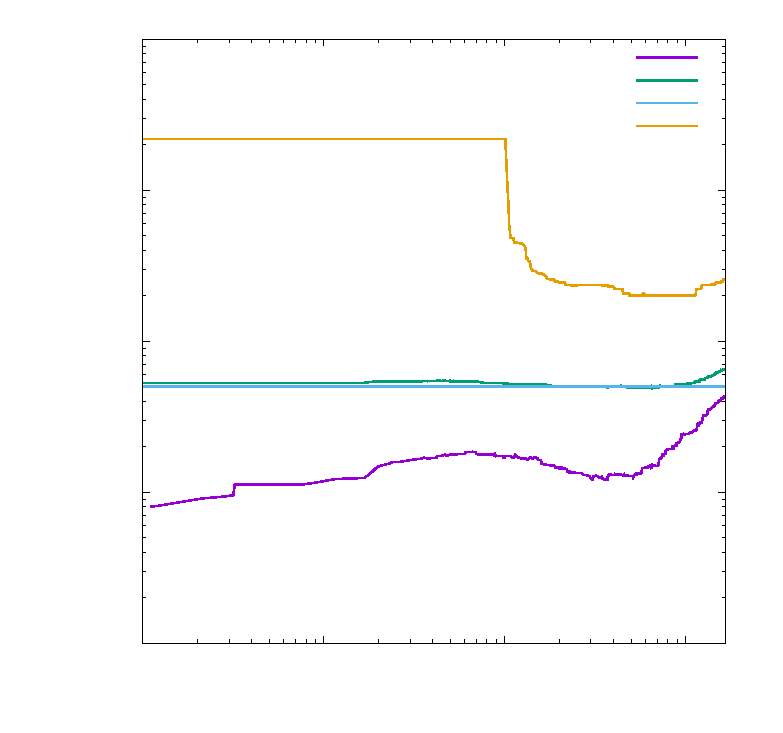
\includegraphics{con}}%
    \gplfronttext
  \end{picture}%
\endgroup
}
  \end{center}
  \caption{Estimating constant population size. For details see
  text.}\label{fig:con}
\end{figure}
\item Next, we simulate under the scenario used in Figure 2b of \cite{liu15:exp}
  with a single, approximately threefold change in population size
  from 7778 to 25636, which occurred 6809 generations ago. Since this simulation includes substantial recombination, we
  replace \ty{ms} by its fast re-implementation, \ty{mspms}
  \citep{kel16:eff}:
\begin{verbatim}
mspms 30 1000 -t 12310 -r 9750 10000000 -eN 0.066 0.3 |
ms2sfs                                                |
epos -u 1.2e-8 -l 10000000 -U                         |
epos2plot > epos2.dat
\end{verbatim}
This takes about 11 minutes. Notice the \ty{-u} option for \ty{epos},
which specifies the mutation rate per generation used by \cite{liu15:exp}, $\mu=1.2\times
10^{-8}$. Plot the result
\begin{verbatim}
gnuplot -p fig2.gp
\end{verbatim}
to get Figure~\ref{fig:2b}. The fit between the median estimated
population size and its true value remains excellent. However, the
variation in estimates is again large, particularly toward the present.
\begin{figure}
  \begin{center}
    \scalebox{0.6}{% GNUPLOT: LaTeX picture with Postscript
\begingroup
  \makeatletter
  \providecommand\color[2][]{%
    \GenericError{(gnuplot) \space\space\space\@spaces}{%
      Package color not loaded in conjunction with
      terminal option `colourtext'%
    }{See the gnuplot documentation for explanation.%
    }{Either use 'blacktext' in gnuplot or load the package
      color.sty in LaTeX.}%
    \renewcommand\color[2][]{}%
  }%
  \providecommand\includegraphics[2][]{%
    \GenericError{(gnuplot) \space\space\space\@spaces}{%
      Package graphicx or graphics not loaded%
    }{See the gnuplot documentation for explanation.%
    }{The gnuplot epslatex terminal needs graphicx.sty or graphics.sty.}%
    \renewcommand\includegraphics[2][]{}%
  }%
  \providecommand\rotatebox[2]{#2}%
  \@ifundefined{ifGPcolor}{%
    \newif\ifGPcolor
    \GPcolortrue
  }{}%
  \@ifundefined{ifGPblacktext}{%
    \newif\ifGPblacktext
    \GPblacktexttrue
  }{}%
  % define a \g@addto@macro without @ in the name:
  \let\gplgaddtomacro\g@addto@macro
  % define empty templates for all commands taking text:
  \gdef\gplbacktext{}%
  \gdef\gplfronttext{}%
  \makeatother
  \ifGPblacktext
    % no textcolor at all
    \def\colorrgb#1{}%
    \def\colorgray#1{}%
  \else
    % gray or color?
    \ifGPcolor
      \def\colorrgb#1{\color[rgb]{#1}}%
      \def\colorgray#1{\color[gray]{#1}}%
      \expandafter\def\csname LTw\endcsname{\color{white}}%
      \expandafter\def\csname LTb\endcsname{\color{black}}%
      \expandafter\def\csname LTa\endcsname{\color{black}}%
      \expandafter\def\csname LT0\endcsname{\color[rgb]{1,0,0}}%
      \expandafter\def\csname LT1\endcsname{\color[rgb]{0,1,0}}%
      \expandafter\def\csname LT2\endcsname{\color[rgb]{0,0,1}}%
      \expandafter\def\csname LT3\endcsname{\color[rgb]{1,0,1}}%
      \expandafter\def\csname LT4\endcsname{\color[rgb]{0,1,1}}%
      \expandafter\def\csname LT5\endcsname{\color[rgb]{1,1,0}}%
      \expandafter\def\csname LT6\endcsname{\color[rgb]{0,0,0}}%
      \expandafter\def\csname LT7\endcsname{\color[rgb]{1,0.3,0}}%
      \expandafter\def\csname LT8\endcsname{\color[rgb]{0.5,0.5,0.5}}%
    \else
      % gray
      \def\colorrgb#1{\color{black}}%
      \def\colorgray#1{\color[gray]{#1}}%
      \expandafter\def\csname LTw\endcsname{\color{white}}%
      \expandafter\def\csname LTb\endcsname{\color{black}}%
      \expandafter\def\csname LTa\endcsname{\color{black}}%
      \expandafter\def\csname LT0\endcsname{\color{black}}%
      \expandafter\def\csname LT1\endcsname{\color{black}}%
      \expandafter\def\csname LT2\endcsname{\color{black}}%
      \expandafter\def\csname LT3\endcsname{\color{black}}%
      \expandafter\def\csname LT4\endcsname{\color{black}}%
      \expandafter\def\csname LT5\endcsname{\color{black}}%
      \expandafter\def\csname LT6\endcsname{\color{black}}%
      \expandafter\def\csname LT7\endcsname{\color{black}}%
      \expandafter\def\csname LT8\endcsname{\color{black}}%
    \fi
  \fi
    \setlength{\unitlength}{0.0500bp}%
    \ifx\gptboxheight\undefined%
      \newlength{\gptboxheight}%
      \newlength{\gptboxwidth}%
      \newsavebox{\gptboxtext}%
    \fi%
    \setlength{\fboxrule}{0.5pt}%
    \setlength{\fboxsep}{1pt}%
\begin{picture}(7200.00,6720.00)%
    \gplgaddtomacro\gplbacktext{%
      \csname LTb\endcsname%%
      \put(1078,704){\makebox(0,0)[r]{\strut{}\large $10^{3}$}}%
      \put(1078,2636){\makebox(0,0)[r]{\strut{}\large $10^{4}$}}%
      \put(1078,4567){\makebox(0,0)[r]{\strut{}\large $10^{5}$}}%
      \put(1078,6499){\makebox(0,0)[r]{\strut{}\large $10^{6}$}}%
      \put(1389,484){\makebox(0,0){\strut{}\large $10^{-1}$}}%
      \put(2361,484){\makebox(0,0){\strut{}\large $10^{0}$}}%
      \put(3333,484){\makebox(0,0){\strut{}\large $10^{1}$}}%
      \put(4305,484){\makebox(0,0){\strut{}\large $10^{2}$}}%
      \put(5277,484){\makebox(0,0){\strut{}\large $10^{3}$}}%
      \put(6249,484){\makebox(0,0){\strut{}\large $10^{4}$}}%
    }%
    \gplgaddtomacro\gplfronttext{%
      \csname LTb\endcsname%%
      \put(198,3601){\rotatebox{-270}{\makebox(0,0){\strut{}\large $N_{\rm e}$}}}%
      \put(4006,154){\makebox(0,0){\strut{}\large Time (Generations)}}%
      \csname LTb\endcsname%%
      \put(5816,6326){\makebox(0,0)[r]{\strut{}\large 5\% quantile}}%
      \csname LTb\endcsname%%
      \put(5816,6106){\makebox(0,0)[r]{\strut{}\large median}}%
      \csname LTb\endcsname%%
      \put(5816,5886){\makebox(0,0)[r]{\strut{}\large 95\% quantile}}%
    }%
    \gplbacktext
    \put(0,0){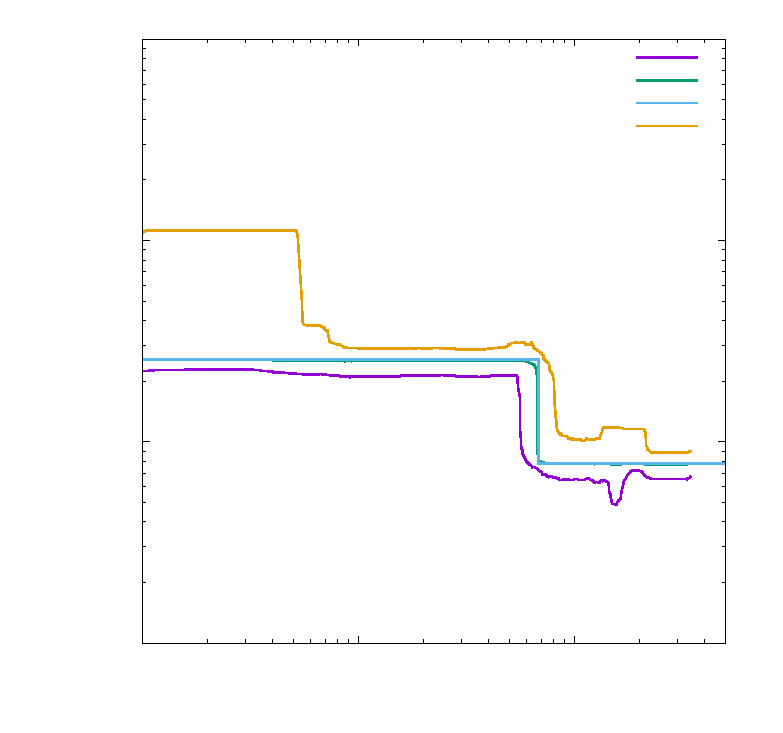
\includegraphics{fig2b}}%
    \gplfronttext
  \end{picture}%
\endgroup
}
  \end{center}
  \caption{Estimating population sizes under a model with one
    instantaneous size change. See text for details.}\label{fig:2b}
\end{figure}
\item As a last example, simulate haplotypes under
  the exponential growth scenario \cite{liu15:exp} used in their
  Figure 2e:
    \small
\begin{verbatim}
mspms 30 1000 -t 432000 -r 340000 10000000 -G 46368 -eN 0.0001027 0.008889 |
ms2sfs                                                                     |
epos -u 1.2e-8 -l 10000000 -U                                              |
epos2plot > epos3.dat
\end{verbatim}
\normalsize
Plot this
\begin{verbatim}
gnuplot -p fig3.gp
\end{verbatim}
to get Figure~\ref{fig:2e}, where the estimation is less
accurate than in the one-step scenario of Figure~\ref{fig:2b}.
This illustrates the difficulty of accurately calculating population size
changes in the recent past.
\begin{figure}
  \begin{center}
    \scalebox{0.6}{% GNUPLOT: LaTeX picture with Postscript
\begingroup
  \makeatletter
  \providecommand\color[2][]{%
    \GenericError{(gnuplot) \space\space\space\@spaces}{%
      Package color not loaded in conjunction with
      terminal option `colourtext'%
    }{See the gnuplot documentation for explanation.%
    }{Either use 'blacktext' in gnuplot or load the package
      color.sty in LaTeX.}%
    \renewcommand\color[2][]{}%
  }%
  \providecommand\includegraphics[2][]{%
    \GenericError{(gnuplot) \space\space\space\@spaces}{%
      Package graphicx or graphics not loaded%
    }{See the gnuplot documentation for explanation.%
    }{The gnuplot epslatex terminal needs graphicx.sty or graphics.sty.}%
    \renewcommand\includegraphics[2][]{}%
  }%
  \providecommand\rotatebox[2]{#2}%
  \@ifundefined{ifGPcolor}{%
    \newif\ifGPcolor
    \GPcolortrue
  }{}%
  \@ifundefined{ifGPblacktext}{%
    \newif\ifGPblacktext
    \GPblacktexttrue
  }{}%
  % define a \g@addto@macro without @ in the name:
  \let\gplgaddtomacro\g@addto@macro
  % define empty templates for all commands taking text:
  \gdef\gplbacktext{}%
  \gdef\gplfronttext{}%
  \makeatother
  \ifGPblacktext
    % no textcolor at all
    \def\colorrgb#1{}%
    \def\colorgray#1{}%
  \else
    % gray or color?
    \ifGPcolor
      \def\colorrgb#1{\color[rgb]{#1}}%
      \def\colorgray#1{\color[gray]{#1}}%
      \expandafter\def\csname LTw\endcsname{\color{white}}%
      \expandafter\def\csname LTb\endcsname{\color{black}}%
      \expandafter\def\csname LTa\endcsname{\color{black}}%
      \expandafter\def\csname LT0\endcsname{\color[rgb]{1,0,0}}%
      \expandafter\def\csname LT1\endcsname{\color[rgb]{0,1,0}}%
      \expandafter\def\csname LT2\endcsname{\color[rgb]{0,0,1}}%
      \expandafter\def\csname LT3\endcsname{\color[rgb]{1,0,1}}%
      \expandafter\def\csname LT4\endcsname{\color[rgb]{0,1,1}}%
      \expandafter\def\csname LT5\endcsname{\color[rgb]{1,1,0}}%
      \expandafter\def\csname LT6\endcsname{\color[rgb]{0,0,0}}%
      \expandafter\def\csname LT7\endcsname{\color[rgb]{1,0.3,0}}%
      \expandafter\def\csname LT8\endcsname{\color[rgb]{0.5,0.5,0.5}}%
    \else
      % gray
      \def\colorrgb#1{\color{black}}%
      \def\colorgray#1{\color[gray]{#1}}%
      \expandafter\def\csname LTw\endcsname{\color{white}}%
      \expandafter\def\csname LTb\endcsname{\color{black}}%
      \expandafter\def\csname LTa\endcsname{\color{black}}%
      \expandafter\def\csname LT0\endcsname{\color{black}}%
      \expandafter\def\csname LT1\endcsname{\color{black}}%
      \expandafter\def\csname LT2\endcsname{\color{black}}%
      \expandafter\def\csname LT3\endcsname{\color{black}}%
      \expandafter\def\csname LT4\endcsname{\color{black}}%
      \expandafter\def\csname LT5\endcsname{\color{black}}%
      \expandafter\def\csname LT6\endcsname{\color{black}}%
      \expandafter\def\csname LT7\endcsname{\color{black}}%
      \expandafter\def\csname LT8\endcsname{\color{black}}%
    \fi
  \fi
    \setlength{\unitlength}{0.0500bp}%
    \ifx\gptboxheight\undefined%
      \newlength{\gptboxheight}%
      \newlength{\gptboxwidth}%
      \newsavebox{\gptboxtext}%
    \fi%
    \setlength{\fboxrule}{0.5pt}%
    \setlength{\fboxsep}{1pt}%
\begin{picture}(7200.00,6720.00)%
    \gplgaddtomacro\gplbacktext{%
      \csname LTb\endcsname%%
      \put(1078,704){\makebox(0,0)[r]{\strut{}\large $10^{3}$}}%
      \put(1078,2636){\makebox(0,0)[r]{\strut{}\large $10^{4}$}}%
      \put(1078,4567){\makebox(0,0)[r]{\strut{}\large $10^{5}$}}%
      \put(1078,6499){\makebox(0,0)[r]{\strut{}\large $10^{6}$}}%
      \put(1210,484){\makebox(0,0){\strut{}\large $10^{0}$}}%
      \put(2445,484){\makebox(0,0){\strut{}\large $10^{1}$}}%
      \put(3679,484){\makebox(0,0){\strut{}\large $10^{2}$}}%
      \put(4914,484){\makebox(0,0){\strut{}\large $10^{3}$}}%
      \put(6148,484){\makebox(0,0){\strut{}\large $10^{4}$}}%
    }%
    \gplgaddtomacro\gplfronttext{%
      \csname LTb\endcsname%%
      \put(198,3601){\rotatebox{-270}{\makebox(0,0){\strut{}\large $N_{\rm e}$}}}%
      \put(4006,154){\makebox(0,0){\strut{}\large Time (Generations)}}%
      \csname LTb\endcsname%%
      \put(5816,6326){\makebox(0,0)[r]{\strut{}\large 5\% quantile}}%
      \csname LTb\endcsname%%
      \put(5816,6106){\makebox(0,0)[r]{\strut{}\large median}}%
      \csname LTb\endcsname%%
      \put(5816,5886){\makebox(0,0)[r]{\strut{}\large expected}}%
      \csname LTb\endcsname%%
      \put(5816,5666){\makebox(0,0)[r]{\strut{}\large 95\% quantile}}%
    }%
    \gplbacktext
    \put(0,0){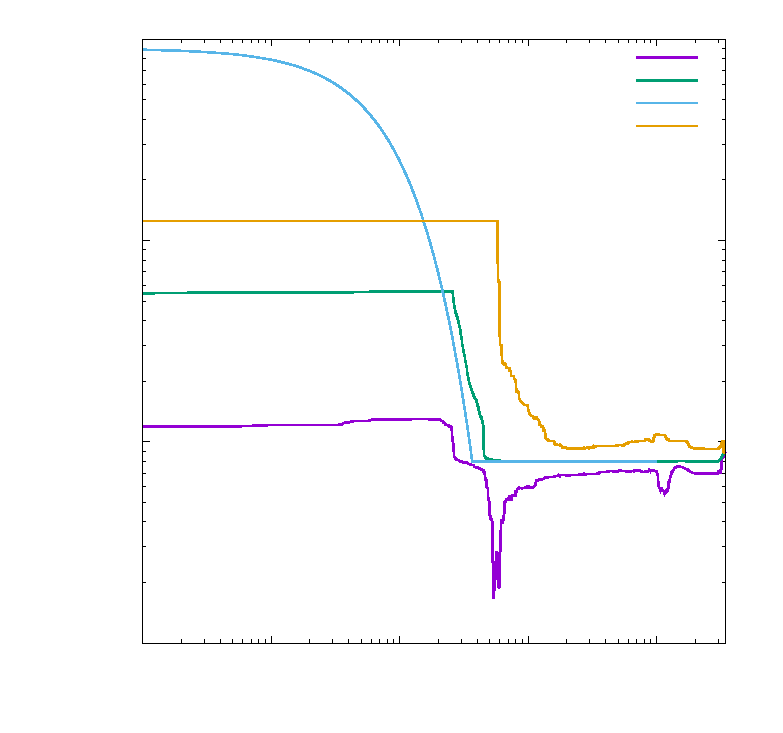
\includegraphics{fig2e}}%
    \gplfronttext
  \end{picture}%
\endgroup
}
  \end{center}
  \caption{Estimating population sizes under an exponential growth
    model. See text for details.}\label{fig:2e}
\end{figure}
\end{itemize}

\subsection{Real Data}
\begin{itemize}
\item As an example for real data, we use a site frequency spectrum obtained from
  the Kap population of \textit{Daphnia pulex}:
\begin{verbatim}
head kap144i.dat 
0	185297
1	1987
2	1138
3	851
4	729
5	672
6	542
7	509
8	459
9	430
\end{verbatim}
Notice the ``zero-class'', which does not appear in the example
spectra in Tables~\ref{tab:sfs}A and B. The zero-class gives the
number of monomorphic sites. If a spectrum contains a zero-class, the
sequence length is the sum of all allele counts, and \ty{epos} does not
require the sequence length to be passed via the \ty{-l}
option. Moreover, the site frequency spectrum of Kap is folded, hence
no \ty{-U}:
\begin{verbatim}
epos ../data/kap144i.dat 
#InputFile:	../data/kap144i.dat
#Polymorphic sites surveyed:	18037
#Monomorphic sites surveyed:	185297
#m = 1; maximum Log(Likelihood): 2149621.403059	{2}
#m = 2; maximum Log(Likelihood): 2150273.656141	{2, 25}
#m = 3; maximum Log(Likelihood): 2150277.188377	{2, 3, 25}
#m = 4; maximum Log(Likelihood): 2150288.578235	{2, 3, 9, 25}
#m = 5; maximum Log(Likelihood): 2150289.124322	{2, 3, 9, 25, 44}
#Final        Log(Likelihood): 2150288.578235
#Level  T[Level]  N[Level]
25      5.48e+04  3.94e+05
9       2.98e+05  7.31e+05
3       2.88e+06  1.72e+06
2       3.16e+06  1.44e+05
\end{verbatim}
\item This only gives a single point estimate, and in the absence of
  further samples it is hard to judge its reliability. However,
  the program \ty{bootSfs}, which is also part of the \ty{sfs} package, implements the bootstrap to investigate the robustness of
  results based on single samples. To run 1000 bootstrap replicates, enter
\begin{verbatim}
bootSfs -i 1000 kap144i.dat | epos | epos2plot > epos4.dat
\end{verbatim}
This takes about five minutes. Plot the result
\begin{verbatim}
gnuplot -p fig4.gp
\end{verbatim}
to get Figure~\ref{fig:kap}.
\begin{figure}
  \begin{center}
    \scalebox{0.6}{% GNUPLOT: LaTeX picture with Postscript
\begingroup
  \makeatletter
  \providecommand\color[2][]{%
    \GenericError{(gnuplot) \space\space\space\@spaces}{%
      Package color not loaded in conjunction with
      terminal option `colourtext'%
    }{See the gnuplot documentation for explanation.%
    }{Either use 'blacktext' in gnuplot or load the package
      color.sty in LaTeX.}%
    \renewcommand\color[2][]{}%
  }%
  \providecommand\includegraphics[2][]{%
    \GenericError{(gnuplot) \space\space\space\@spaces}{%
      Package graphicx or graphics not loaded%
    }{See the gnuplot documentation for explanation.%
    }{The gnuplot epslatex terminal needs graphicx.sty or graphics.sty.}%
    \renewcommand\includegraphics[2][]{}%
  }%
  \providecommand\rotatebox[2]{#2}%
  \@ifundefined{ifGPcolor}{%
    \newif\ifGPcolor
    \GPcolortrue
  }{}%
  \@ifundefined{ifGPblacktext}{%
    \newif\ifGPblacktext
    \GPblacktexttrue
  }{}%
  % define a \g@addto@macro without @ in the name:
  \let\gplgaddtomacro\g@addto@macro
  % define empty templates for all commands taking text:
  \gdef\gplbacktext{}%
  \gdef\gplfronttext{}%
  \makeatother
  \ifGPblacktext
    % no textcolor at all
    \def\colorrgb#1{}%
    \def\colorgray#1{}%
  \else
    % gray or color?
    \ifGPcolor
      \def\colorrgb#1{\color[rgb]{#1}}%
      \def\colorgray#1{\color[gray]{#1}}%
      \expandafter\def\csname LTw\endcsname{\color{white}}%
      \expandafter\def\csname LTb\endcsname{\color{black}}%
      \expandafter\def\csname LTa\endcsname{\color{black}}%
      \expandafter\def\csname LT0\endcsname{\color[rgb]{1,0,0}}%
      \expandafter\def\csname LT1\endcsname{\color[rgb]{0,1,0}}%
      \expandafter\def\csname LT2\endcsname{\color[rgb]{0,0,1}}%
      \expandafter\def\csname LT3\endcsname{\color[rgb]{1,0,1}}%
      \expandafter\def\csname LT4\endcsname{\color[rgb]{0,1,1}}%
      \expandafter\def\csname LT5\endcsname{\color[rgb]{1,1,0}}%
      \expandafter\def\csname LT6\endcsname{\color[rgb]{0,0,0}}%
      \expandafter\def\csname LT7\endcsname{\color[rgb]{1,0.3,0}}%
      \expandafter\def\csname LT8\endcsname{\color[rgb]{0.5,0.5,0.5}}%
    \else
      % gray
      \def\colorrgb#1{\color{black}}%
      \def\colorgray#1{\color[gray]{#1}}%
      \expandafter\def\csname LTw\endcsname{\color{white}}%
      \expandafter\def\csname LTb\endcsname{\color{black}}%
      \expandafter\def\csname LTa\endcsname{\color{black}}%
      \expandafter\def\csname LT0\endcsname{\color{black}}%
      \expandafter\def\csname LT1\endcsname{\color{black}}%
      \expandafter\def\csname LT2\endcsname{\color{black}}%
      \expandafter\def\csname LT3\endcsname{\color{black}}%
      \expandafter\def\csname LT4\endcsname{\color{black}}%
      \expandafter\def\csname LT5\endcsname{\color{black}}%
      \expandafter\def\csname LT6\endcsname{\color{black}}%
      \expandafter\def\csname LT7\endcsname{\color{black}}%
      \expandafter\def\csname LT8\endcsname{\color{black}}%
    \fi
  \fi
    \setlength{\unitlength}{0.0500bp}%
    \ifx\gptboxheight\undefined%
      \newlength{\gptboxheight}%
      \newlength{\gptboxwidth}%
      \newsavebox{\gptboxtext}%
    \fi%
    \setlength{\fboxrule}{0.5pt}%
    \setlength{\fboxsep}{1pt}%
\begin{picture}(7200.00,6720.00)%
    \gplgaddtomacro\gplbacktext{%
      \csname LTb\endcsname%%
      \put(1078,704){\makebox(0,0)[r]{\strut{}\large $10^{4}$}}%
      \put(1078,2153){\makebox(0,0)[r]{\strut{}\large $10^{5}$}}%
      \put(1078,3601){\makebox(0,0)[r]{\strut{}\large $10^{6}$}}%
      \put(1078,5050){\makebox(0,0)[r]{\strut{}\large $10^{7}$}}%
      \put(1078,6499){\makebox(0,0)[r]{\strut{}\large $10^{8}$}}%
      \put(2756,484){\makebox(0,0){\strut{}\large $10^{4}$}}%
      \put(4308,484){\makebox(0,0){\strut{}\large $10^{5}$}}%
      \put(5860,484){\makebox(0,0){\strut{}\large $10^{6}$}}%
    }%
    \gplgaddtomacro\gplfronttext{%
      \csname LTb\endcsname%%
      \put(198,3601){\rotatebox{-270}{\makebox(0,0){\strut{}\large $N_{\rm e}$}}}%
      \put(4006,154){\makebox(0,0){\strut{}\large Time (Generations)}}%
      \csname LTb\endcsname%%
      \put(5816,6326){\makebox(0,0)[r]{\strut{}\large 5\% quantile}}%
      \csname LTb\endcsname%%
      \put(5816,6106){\makebox(0,0)[r]{\strut{}\large median}}%
      \csname LTb\endcsname%%
      \put(5816,5886){\makebox(0,0)[r]{\strut{}\large 95\% quantile}}%
    }%
    \gplbacktext
    \put(0,0){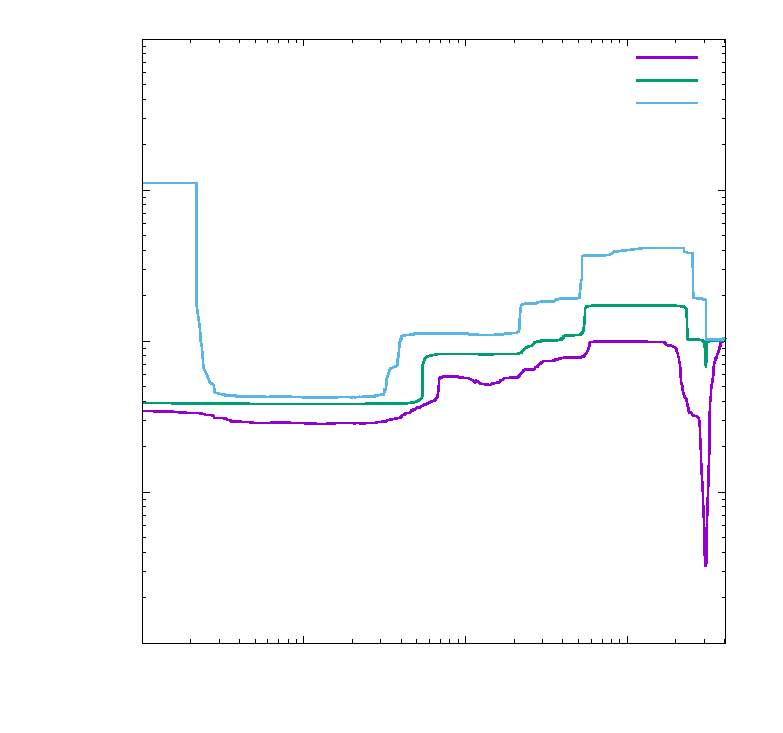
\includegraphics{kap}}%
    \gplfronttext
  \end{picture}%
\endgroup
}
  \end{center}
  \caption{Estimating the population size of the \textit{D. pulex} Kap
    population.}\label{fig:kap}
\end{figure}
\end{itemize}

\section{The Averge Age of an Allele}
\begin{itemize}
  \item To start with a simple example, simulate a site frequency spectrum with $n=2$,
\begin{verbatim}
ms 2 1 -t 10 | ms2sfs > test.sfs
\end{verbatim}
estimate the population size,
\begin{verbatim}
epos -U -l 1000 test.sfs
#InputFile:	test.sfs
#Polymorphic sites surveyed:	8
#Monomorphic sites surveyed:	992
#m = 1; maximum Log(Likelihood): 5861.160855	{2}
#m = 2; no improvement
#Final        Log(Likelihood): 5861.160855
#Level  T[Level]  N[Level]
2       8.00e+05  4.00e+05
\end{verbatim}
and the age of singletons
\begin{verbatim}
epos -U -l 1000 test.sfs | epos2ages -n 2
#r  A[r]    V(A[r])      P[r]
1   800000  2.55999e+17  400000
\end{verbatim}
where the second column gives their average age as $8\times 10^5$,
twice the population size. Since \ty{epos2ages} follows the convention
of measuring time in units of $2N$ generations, this is the correct
result. The other two output columns of \ty{epos2ages} are the
variance of the age, and the average population size experienced by
the allele, which again agrees with the previous \ty{epos} result.
\item For larger samples of 30 haplotypes the population sizes might look like this
\begin{verbatim}
ms 30 1 -t 1000 | ms2sfs | tee test.sfs | epos -U -l 10000000 
#InputFile:	stdin
#Polymorphic sites surveyed:	2467
#Monomorphic sites surveyed:	9997533
#m = 1; maximum Log(Likelihood): 151151463.358135	{2}
#m = 2; maximum Log(Likelihood): 151151519.931473	{2, 10}
#m = 3; maximum Log(Likelihood): 151151602.167420	{2, 3, 10}
#m = 4; no improvement
#Final        Log(Likelihood): 151151602.167420
#Level  T[Level]  N[Level]
10      1.82e+03  5.84e+03
3       2.75e+03  6.03e+02
2       1.04e+04  3.80e+03
\end{verbatim}
and the corresponding allele sizes
\begin{verbatim}
epos -U -l 10000000 test.sfs | epos2ages -n 30
#r  A[r]     V(A[r])      P[r]
1   938.084  4.72335e+06  5148.63
2   1688.78  1.07603e+07  4867.1
3   2491.19  1.8408e+07   4617.42
...
29  10354.9  5.82315e+07  3868.34
\end{verbatim}
\item Finally, we can estimate the average age of alleles for the Kap
  population:
\begin{verbatim}
epos2ages -n 144 data/kap144i.out
#r   A[r]         V(A[r])      P[r]
1    227105       3.89154e+11  1.3394e+06
2    374758       6.05738e+11  1.35968e+06
3    483237       7.47685e+11  1.37444e+06
...
143  3.16639e+06  1.94476e+12  1.47763e+06
\end{verbatim}  
\end{itemize}

\section{Change Log}
\begin{itemize}
\item Version 0.1 (Oct. 25, 2017)
  \begin{itemize}
  \item First running version based on the GSL.
  \end{itemize}
\item Version 0.2 (Oct 26, 2017)
  \begin{itemize}
    \item Used \ty{LAPACKE\_dgesv} in \ty{getPopSizes}; makes no
      difference compared to the previous version.
  \end{itemize}
\item Version 0.3 (Oct 26, 2017)
  \begin{itemize}
    \item Used \ty{LAPACKE\_dgesvx} in \ty{getPopSizes}; makes no
      difference compared to previous version.
  \end{itemize}
\item Version 0.4 (Oct 27, 2017)
  \begin{itemize}
  \item Allow construction of SFS based on \ty{-t} switch.
  \item Allow switching between the GSL algorithm (\ty{-g}) and the
    default LAPACK algorithm. 
  \end{itemize}
\item Version 0.5 (November 2, 2017)
  \begin{itemize}
    \item Allow the straight usage of the trapezoid matrix for solving
      the system (\ty{-T}).
    \item Print out coefficient matrix (\ty{-p}).
  \end{itemize}
\item Version 0.6 (November 10, 2017)
  \begin{itemize}
  \item Use \ty{long double} in \ty{getPopSizesTri2}; did not help.
  \end{itemize}
\item Version 0.7 (November 10, 2017)
  \begin{itemize}
    \item Implement Peter Pfaffelhuber's formula; working only partially.
  \end{itemize}
\item Version 0.8 (November 10, 2017)
  \begin{itemize}
    \item Peter's equation (6) is working.
  \end{itemize}
\item Version 0.9 (November 10, 2017)
  \begin{itemize}
  \item Peter's equation in arbitrary precision in MPFR
    library. Numerical stability achieved with 329 bits per number.
  \end{itemize}
\item Version 0.10 (November 30, 2017)
  \begin{itemize}
  \item Implemented equation (3) from Peter's memo dated Nov. 13. Not
    working.
  \end{itemize}
\item Version 0.11 (December 1, 2017)
  \begin{itemize}
  \item Implemented revised equation (3) from Peter's memo dated Nov. 30. Not
    working.
  \end{itemize}
\item Version 0.12 (December 15, 2017)
  \begin{itemize}
    \item Implemented Estimator 2.1 from Peter's memo dated Dec. 2,
      2017. Code is running, but the results look odd.
  \end{itemize}
\item Version 0.13 (December 16, 2017)
  \begin{itemize}
  \item Fixed the implementation of Estimator 2.1; results OK now.
  \end{itemize}
\item Version 0.14 (December 18, 2017)
  \begin{itemize}
  \item Implemented optimization strategy for folded SFS; working.
  \item Implemented optimization strategy for unfolded/even SFS;
    working.
  \item Implemented optimization strategy for folded/odd SFS; not
    working yet.
  \end{itemize}
\item Version 0.15 (December 18, 2017)
  \begin{itemize}
  \item Fixed error in search for optimal number of steps.
  \end{itemize}
\item Version 0.16 (December 19, 2017)
  \begin{itemize}
  \item Fixed error in left-hand side of folded/odd equation; working.
  \item Changed search strategy.
  \item Changed default value of \ty{-d} from $10^{-6}$ to $10^{-3}$.
  \item Simplified user interface.
  \item Included set of test cases (\ty{test.sh}).
  \end{itemize}
  \item Version 0.17 (December 20, 2017)
  \begin{itemize}
  \item Fixed searching routine.
  \item Changed default value of \ty{-d} from $10^{-3}$ to $10^{-2}$.
  \item Included addition of the $\lambda$-factor; seems to make no difference.
  \end{itemize}
\item Version 0.18 (December 20, 2017)
  \begin{itemize}
  \item Fixed the $\lambda$-factor; computation is now much
    stabilized.
  \end{itemize}
\item Version 0.19 (January 11, 2018)
  \begin{itemize}
  \item Included the $\lambda$-factor in the computation of
    $\Psi$. Computations now applicable to real data.
  \item Changed the default-value of $\lambda$ from $10^{-7}$ to $10^{-5}$.
  \end{itemize}
\item Version 0.20 (January 11, 2018)
  \begin{itemize}
  \item Consider zero-class mutations in computation, if present.
  \item Changed default $\lambda$ to $2\times 10^{-5}$ to get all data
    sets to run.
  \end{itemize}
\item Version 0.21 (January 13, 2018)
  \begin{itemize}
    \item Reverted output of levels, going from the present into the
      past.
    \item Default output is now as a function of times instead as a
      function of levels.
    \item Included ``step-wise'' option for plotting times and levels.
    \item Fixed time computation.
    \item Included error message for negative population sizes.
    \item Removed memory leaks and other subtle bugs using \ty{valgrind}.
  \end{itemize}
\item Version 0.22 (January 16, 2018)
  \begin{itemize}
    \item Fixed important bug in function foldedEpsi, where variable
      \ty{b} was computed as a function of \verb+sfs->f[n/2]+ instead
      of, now \verb+sfs->f[n/2-1]+.
  \end{itemize}
\item Version 0.23 (January 16, 2018)
  \begin{itemize}
  \item Search for optimal $\lambda$.
  \item Allow arbitrary level as first entry in level list.
  \item Output $\lambda$, $\Psi$, and the levels added to make it
    easier to follow the program.
  \item Reduced program to folded/even case.
  \end{itemize}
\item Version 0.23 (January 17, 2018)
  \begin{itemize}
  \item Catch GSL-exceptions.
  \item Changed output format
  \end{itemize}
\item Version 0.24 (January 18, 2018)
  \begin{itemize}
  \item Not quite sure what changed.
  \end{itemize}
\item Version 0.25 (January 18, 2018)
  \begin{itemize}
  \item Fixed bug in computation of the $\lambda$-term in
    \ty{foldedEpsi}.
  \end{itemize}
\item Version 0.26 (January 19, 2018)
  \begin{itemize}
  \item Set $\lambda=0$ and add levels until negative population sizes
    appear. This is fast and appears to be effective.
  \end{itemize}
\item Version 0.27 (January 24, 2018)
  \begin{itemize}
  \item Output number of polymorphic and monomorphic sites surveyed.
  \end{itemize}
\item Version 0.28 (???)
\item Version 0.29 (January 28, 2018)
  \begin{itemize}
  \item Fixed missing resetting of times during iteration over files.
  \item Removed superfluous option for step-wise output (\ty{-s}).
  \item Output name of input file.
  \item Removed inclusion of \ty{mpfr.h} from \ty{epos.c}.
  \item Removed search for the initial level to add; by definition
    this must be 2, i. e. one population size for the entire coalescent.
  \end{itemize}
\item Version 0.30 (January 31, 2018)
  \begin{itemize}
  \item Fixed computation of the mutation rate. Previously I
    multiplied the per site mutation rate with the number of
    monomorphic positions. Now it is mutated by the number of all
    positions.
  \item Added bootstrapping.
  \end{itemize}
\item Version 0.31 (February 1, 2018)
  \begin{itemize}
    \item Computation of mutation rate was correct in previous
      version, after all, so reverted to that.
  \end{itemize}
\item Version 0.32 (February 7, 2018)
  \begin{itemize}
    \item Introduced the \ty{-m} switch.
  \end{itemize}
\item Version 0.33 (February 7, 2018)
  \begin{itemize}
    \item Fixed $\delta$ computation in function \ty{delta} in
      \ty{util.c}. This reduces the computation for $m=1$ to
      Watterson's estimator, as expected.
  \end{itemize}
\item Version 0.34 (February 9, 2018)
  \begin{itemize}
    \item Reintroduced unfolded spectrum (\ty{-u}) and compared to the equations
      in Peter's memo of December 19, 2017.
    \item Reintroduced $\lambda$ and set it by default to $10^{-7}$.
    \item Reintroduced $\delta$ and set it by default to $0.0$.
    \item Fixed sample size computation at the end of \ty{sfs.c}.
  \end{itemize}
\item Version 0.35 (February 9, 2018)
  \begin{itemize}
  \item Introduced estimation of $\lambda=1./\mu/\texttt{args->f}$.
  \end{itemize}
\item Version 0.36 (February 14, 2018)
  \begin{itemize}
    \item Changed setting of $\lambda$ to
      $\lambda=\mu\times\texttt{args->f}$. By default
      $\texttt{args->f}=1$.
  \end{itemize}
\item Version 0.37 (February 16, 2018)
  \begin{itemize}
    \item Fixed sample size computation for folded/even in function
      \ty{getSfs} in \ty{sfs.c}.
  \end{itemize}
\item Version 0.38 (February 16, 2018)
  \begin{itemize}
  \item Included working \ty{-m} switch.
  \end{itemize}
\item Version 0.39 (February 19, 2018)
  \begin{itemize}
  \item Fixed passing of $\lambda$ in iterated runs.
  \item Fixed numerical underflow when multiplying with $\lambda$ in
    \ty{foldedEpsi} in \ty{foldedE.c}.
  \item Fixed numerical underflow when multiplying with $\lambda$ in
    \ty{psi} in \ty{unfolded.c}
  \item Included check for positive $\Psi$ in both cases.
  \item Expanded verbose output.
  \end{itemize}
\item Version 0.40 (February 21, 2018)
  \begin{itemize}
  \item Fixed error in \ty{foldedEpsi} in \ty{foldedE.c}
  \item Removed \ty{if(m > 1)} from \ty{getCoeffMat} in
    \ty{foldedE.c}.
  \item Switched \ty{n/2} in \ty{foldedEpsi} to \ty{n/2.}.
  \item Ensured that \ty{sfs->u} is always set to a value in
    \ty{getSfs}.
  \item Replace \verb+u = args->u+ by \verb+u = sfs->u+ in
    \ty{getCoeffMat} in \ty{unfolded.c}.
  \item Re-implemented \ty{foldedEpsi} in \ty{foldedE.c}
  \end{itemize}
\item Version 0.41 (February 22, 2018)
  \begin{itemize}
    \item Changed \ty{4.*u*(n/2.)} to \ty{4.*u/(n/2.)} in
      \ty{foldedEpsi} in \ty{foldedE.c}. This was a bug in the
      computation of $\Psi$ for the folded/even case.
  \end{itemize}
\item Version 0.42 (February 22, 2018)
  \begin{itemize}
    \item Removed line \ty{prevMinPsi = DBL\_MAX} in \ty{foldedE} in \ty{foldedE.c}.
  \end{itemize}
\item Version 0.43 (February 22, 2018)
  \begin{itemize}
    \item Added diagnostic output in case negative population sizes
      are found.
  \end{itemize}
\item Version 0.44 (February 22, 2018)
  \begin{itemize}
  \item $\Psi$ now also reported if only one level is included.
  \end{itemize}
\item Version 0.45 (February 23, 2018)
  \begin{itemize}
  \item Included the \ty{-n} option to allow negative population
    sizes.
  \end{itemize}
\item Version 0.46 (February 23, 2018)
  \begin{itemize}
    \item Fixed \ty{if(change > args->d)}-phrase in \ty{unfolded} and
      \ty{foldedE}. This lacked re-computation of the population sizes
      with the best new level added, and assignment of $\Psi$.
  \end{itemize}
\item Version 0.47 (February 26, 2018)
  \begin{itemize}
    \item Reorganized code to remove duplication. The searching for
      best population sizes is now done in only one place,
      \ty{getPopSizes} in \ty{popSizes.c}.
    \item Added printing of intermediate population sizes if the
      \ty{-V} option is used.
  \end{itemize}
\item Version 0.48 (March 2, 2018)
  \begin{itemize}
  \item Multi-threaded version.
  \end{itemize}
\item Version 0.49 (March 6, 2018)
  \begin{itemize}
  \item Reverted to single-threaded behavior by removing \ty{-t} from
    the options list and setting it to 1 in the background. This avoids the occasional
    race-conditions observed with the multi-threaded version.
  \end{itemize}
\item Version 0.50 (March 14, 2018)
  \begin{itemize}
  \item Find number of levels through cross-validation (\ty{-c}).
  \end{itemize}
\item Version 0.51 (March 14, 2018)
  \begin{itemize}
  \item Find lambda through cross-validation (\ty{-L}).
  \end{itemize}
\item Version 0.52 (March 17, 2018)
  \begin{itemize}
    \item Include reporting of negative population sizes in verbose
      output (\ty{-V}).
    \item Changed     \ty{prevMinPsi = prevMinPsi;} in
      \ty{getPopSizes} to \ty{prevMinPsi = currMinPsi;}.
  \end{itemize}
\item Version 0.53 (April 7, 2018)
  \begin{itemize}
  \item Always allow negative population sizes.
  \item Cross-validation by default.
  \item $\lambda=0$ by default.
  \item If negative population sizes are found, the program searches
    for optimal $\lambda$ by going through $\lambda=0..\mu$. This is
    slow and would need to be optimized in future versions.
  \item Added Scripts for extracting quantiles from \ty{epos} output.
  \end{itemize}
\item Version 0.54 (April 11, 2018)
  \begin{itemize}
    \item Fixed array out-of-bounds error in \ty{shuffleArr} in \ty{sfs.c}.
  \end{itemize}
\item Version 0.55 (April 12, 2018)
  \begin{itemize}
    \item ``Unfolded'' mode not working; so I removed that option for now.
  \end{itemize}
\item Version 0.56 (May 31, 2018)
  \begin{itemize}
  \item Fixed Error in documentation.
  \end{itemize}
\item June 13, 2018
  \begin{itemize}
    \item Posted \ty{epos} on \ty{github}. Please refer to the commit
      messages for details on subsequent changes.
  \end{itemize}
\end{itemize}
\bibliography{/home/haubold/References/references}
\end{document}

